\setlength{\columnsep}{3pt}
\begin{flushleft}
	\bigskip
	\begin{itemize}
		\item Commands read input using standard input device and produce output on standard output device.
		\item Standard input device: \textbf{Keyboard}
		\item Standard output device: \textbf{Screen} or \textbf{Desktop} or \textbf{Terminal window}
		\begin{figure}[h!]
			\centering
			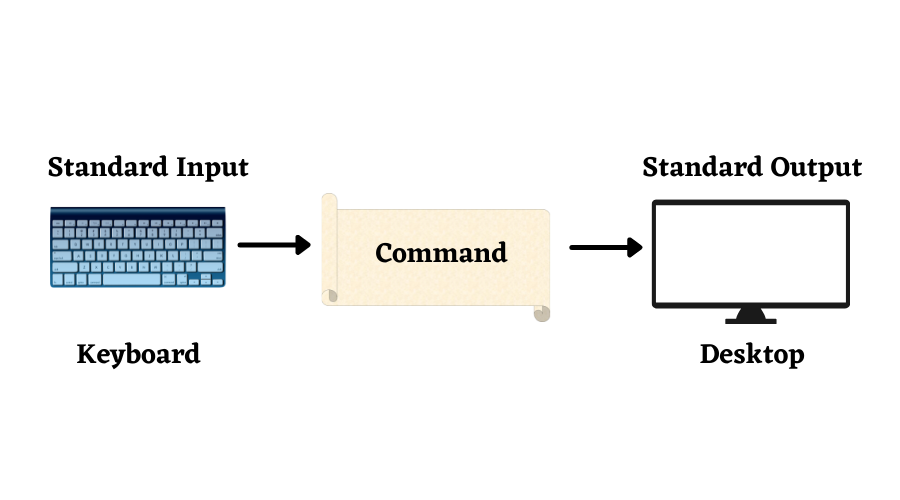
\includegraphics[scale=.5]{content/chapter7/images/std_in_out.png}
			\caption{Standard input and output device}
			\label{fig:path}
		\end{figure}
	\end{itemize}
	
\end{flushleft}

\newpage

